\documentclass[12pt]{article}
\usepackage[utf8]{inputenc}
\usepackage[margin=.7in]{geometry}
\usepackage{amssymb}
\usepackage{amsmath}
\usepackage{mathtools}
\usepackage{amsthm}
\usepackage{setspace}
\usepackage{cancel}
\usepackage{bbm}
\usepackage{pgfplots}
\usetikzlibrary{arrows, calc, patterns, shapes}
  \pgfplotsset{compat=1.15}
\renewcommand{\baselinestretch}{1.25}
\newcommand\sbullet[1][.5]{\mathbin{\vcenter{\hbox{\scalebox{#1}{$\bullet$}}}}}
\newcommand{\indep}{\perp \hspace{-.5 em} \perp}
\def\E{\mathbb{E}}
\def\e{\mathcal{E}}
\def\d{\mathcal{D}}
\def\I{I_n}
\def\l{\ell}
\def\sumn{\sum^n_{i=1}}
\def\i{\mathcal{J}}
\def\x{\mathbf{X}}
\newcommand{\til}[1]{\underset{\sim}{#1}}
\newcommand\expp[1]{\exp\bigg\{#1\bigg\}}
\newcommand\der[2]{\frac{\partial #1}{\partial #2}}
\newcommand{\ds}{\displaystyle}
\newtheorem{case}{Case}
\newtheorem{note}{Note}

\theoremstyle{definition}
\newtheorem{definition}{Definition}

\newtheorem{example}{Example}[section]

\let\inf\infty
\title{Math 410}
\author{--- }
\date{September 2019}

\begin{document}

\maketitle
\tableofcontents{}
\pagebreak

\section{Necessary Background }

\subsection{Brief Introduction to Bayesian Networks}
The goal of Bayesian Networks is to represent a joint distribution over a set of random variables using a directed acyclic graph. Let $\mathcal{D}=(V,E)$ be such a graph. The set of nodes $V$ will represent random variables and the set of edges $E$ will correspond to the direct influence between two nodes. Intuitively, edge orientation can be interpreted at a causal relation between two rvs.

\noindent
When working with Bayesian Networks, nodes (rvs) are independent from other nodes given their immediate parents. This is referred to as the he \textbf{Markov property}.
\begin{center}
\tikzset{every picture/.style={line width=0.75pt}}
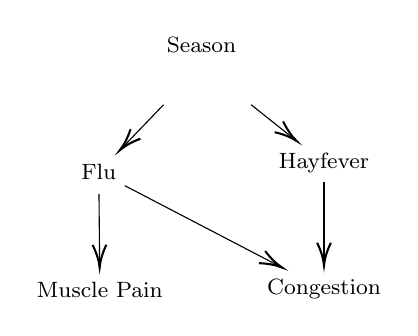
\begin{tikzpicture}[x=0.75pt,y=0.75pt,yscale=-1,xscale=1]
\draw (225,56) node  [align=left] {{\footnotesize Season}\\};
\draw (175.5,107.5) node  [align=left] {{\footnotesize Flu}};
\draw (284,103) node  [align=left] {{\footnotesize Hayfever}};
\draw (284,164) node  [align=left] {{\footnotesize Congestion}};
\draw (176,164) node  [align=left] {{\footnotesize Muscle Pain}};
\draw    (206.74,75) -- (186.98,95.56) ;
\draw [shift={(185.59,97)}, rotate = 313.87] [color={rgb, 255:red, 0; green, 0; blue, 0 }  ][line width=0.75]    (10.93,-3.29) .. controls (6.95,-1.4) and (3.31,-0.3) .. (0,0) .. controls (3.31,0.3) and (6.95,1.4) .. (10.93,3.29)   ;
\draw    (248.85,75) -- (269.25,91.25) ;
\draw [shift={(270.82,92.5)}, rotate = 218.54] [color={rgb, 255:red, 0; green, 0; blue, 0 }  ][line width=0.75]    (10.93,-3.29) .. controls (6.95,-1.4) and (3.31,-0.3) .. (0,0) .. controls (3.31,0.3) and (6.95,1.4) .. (10.93,3.29)   ;
\draw    (188,114.01) -- (262.06,152.58) ;
\draw [shift={(263.84,153.5)}, rotate = 207.51] [color={rgb, 255:red, 0; green, 0; blue, 0 }  ][line width=0.75]    (10.93,-3.29) .. controls (6.95,-1.4) and (3.31,-0.3) .. (0,0) .. controls (3.31,0.3) and (6.95,1.4) .. (10.93,3.29)   ;
\draw    (175.59,118) -- (175.89,151.5) ;
\draw [shift={(175.91,153.5)}, rotate = 269.49] [color={rgb, 255:red, 0; green, 0; blue, 0 }  ][line width=0.75]    (10.93,-3.29) .. controls (6.95,-1.4) and (3.31,-0.3) .. (0,0) .. controls (3.31,0.3) and (6.95,1.4) .. (10.93,3.29)   ;
\draw    (284,112.5) -- (284,150.5) ;
\draw [shift={(284,152.5)}, rotate = 270] [color={rgb, 255:red, 0; green, 0; blue, 0 }  ][line width=0.75]    (10.93,-3.29) .. controls (6.95,-1.4) and (3.31,-0.3) .. (0,0) .. controls (3.31,0.3) and (6.95,1.4) .. (10.93,3.29)   ;
\end{tikzpicture}
\end{center}
By the Markov property,  BN above represents the following joint probability:
$$P(s,f,h,m,c)=P(s)P(f|s)P(h|s)P(m|f)P(c|f,h)$$

\subsection{Monoid}
A set $S$ with a binary operator $\bullet : S \times S \rightarrow S $ is a \textbf{monoid} if it satisfies the following properties:
\begin{itemize}
    \item \textbf{Associativity:} $\forall a,b,c \in S, (a\bullet b)\bullet c = a \bullet (b\bullet c)$ 
    \item \textbf{Identity Element} $\exists e \in S\ \  s.t.\  \forall a\in S, e \bullet a =a \bullet e = a$
\end{itemize}

\subsection{Semiring}
A \textbf{semiring} $(R,\bigvee,\cdot)$ is defined by a set $R$ and two of its operators with the following properties:
\begin{itemize}
    \item $(R,\bigvee) $ is a commutative monoid with identity 0
    \item $(R,\cdot)$ is a monoid with identity 1
\end{itemize}
In the contex of max-linear models, we will be using $\bigvee$ as the max operator, and $\cdot$ as the matrix product.

\section{Introduction to Max-Linear Models}
\subsection{Recursive Structural Equation Model}
Given a DAG $\mathcal{D}=(V,E)$ with nodes $V=\{1,\hdots, d\}$ and edges $E=\{(k,i):i \in V \ \text{and } K \in pa(i)\}$, we define a \textbf{recursive structural equation model} to be any function $$X_i=f_i(X_{pa(i)},Z_i)$$

\begin{itemize}
    \item with $ \ds pa(i)$ denoting the direct parents of node $i$ in $\mathcal{D}$
    \item $f_i$ as a real valued measurable function
    \item $\ds \{ Z_1, \hdots , Z_d\}$ as independent noise variables\footnote{The distribution $\mathbf{X}$ is uniquely determined by these noise variables}
\end{itemize}
By analyzing the set of equations, $\mathbf{X}= (X_1, \hdots, X_d)$, we can see why this model has its name. $\x$ is recursively generated and, through parentage, the generation of each successive $X_i$ is driven by the structure of the graph.

\noindent Let $nd(i)$ denote the set of non-descendants of $i$ then, by construction, 
$$X_i \indep X_{nd(i)\setminus pa(i)}|X_{pa(i)} \ \ \ i=1,\hdots, d$$
 which means that the distribution on $\mathbf{X}$ is Markov with respect to $\mathcal{D}$.
 
\subsection{Recursive Max-Linear Model}
 This model is motivated by its applications to risk analysis and the tendency of risk to propagate through a network. The \textbf{recursive max-linear model} $\x=(X_1,\hdots, X_d)$ on a DAG $\mathcal{D}$ is defined as:
$$X_i:= \bigvee_{k\in pa(i)}c_{ki}X_k \vee c_{ii}Z_i\ \ \  i=1,\hdots,d$$
\begin{itemize}
    \item $\ds \{c_{ki} \forall i \in V \text{and } k \in pa(i)\cup\{i\}\}$ as positive weights 
    \item $\{Z_1, \hdots Z_d\}$ as independent, non negative rvs with positive and infinite support.
\end{itemize}
The weights represent relative quantities that a risk originates with a certain proportion in different ancestors.

\subsubsection{Max-Linear Coefficient Matrix}
\noindent This model can be re-written in the form $$X_i:= \bigvee_{j=1}^db_{ji}Z_j\ \ \  i=1,\hdots,d$$
$B=(b_{ij})_{d\times d}$ is a matrix with non-negative entries called the \textbf{max linear coefficient matrix} of $\x$ and its entries are dubbed \textbf{max-linear coefficients}. The construction of the matrix $B$ is fairly intuitive. First, for any two nodes $(j,i)$ we assign a weight to every path $p= [j=k_0\rightarrow k_1\rightarrow \hdots \rightarrow k_n=i]$. This weight is equal to the edge product allong the path $p$ multiplied by the noise variable (denoted $Z_j$) associated with the starting node $j$. Below is an equation that might assist in visualizing the edge product $d_{ji}(p)$:
$$d_{ji}(p):=c_{k_0,k_0}\cdot c_{k_0,k_1}\cdot\hdots\cdot c_{k_{n-2},k_{n-1}}\cdot c_{k_{n-1},k_n}=c_{k_0,k_0}\prod_{l=0}^{n-1}c_{k_l,k_{l+1}}$$
Let $an(i)$ denote the ancestors of a node and $P_{ji}$ denote all possible paths from node $j$ to node $i$. Then, the ML coefficients for any $i\in V$ are given by:
$$b_{ji}=\bigvee_{p\in P_{ji}}d_{ji} \text{ for }j\in an(i);b_{ii}\in c_{ii}; b_{ji}=0 \text{ for } j \in V \setminus (an(i)\cup \{i\})$$
\begin{itemize}
    \item The coefficient between any two nodes $(j,i)$ is given by the path with the largest weight
    \item The coefficient between a node $i$ and itself is simply the weight $c_{ii}$
    \item The coefficient between any two nodes with no path between them is $0$
\end{itemize}
From our construction, our new model for $X_i$ comes with a slightly new explanation. In \textit{"pseudo stats"}, the model is given by :
$$X_i=\max_{\text{for all nodes }j\in V}\bigg( \max(\text{path weight between nodes }i \text{ and }j ) * \text{noise associated to }j\bigg) $$

\textbf{SKIPPED THE SOME FORMALITIES (proof its an rsem, graph structure stuff, complexity reduction, ordering ...) }
\pagebreak

\subsubsection{Example of Max-Linear Model}
Let $\d=(V,E)=(\{1,2,3,4\}, \{(1,2),(1,3), (2,4),(3,4)\})$, and $C=\{c_{ik}: i\in V, k\in pa(i)\}$. Now, let us build the recursive ML model $\x= (X_1,X_2,X_3,X_4)$\\
\begin{minipage}{0.5 \linewidth}
$ 
\begin{aligned}[t] 
X_1&= c_{11}Z_1\\
X_2&= c_{12}X_1\vee c_{22}Z_2 =c_{12}c_{11}Z_1 \vee c_{22}Z_2\\
X_3&= c_{13}X_1\vee c_{33}Z_3 =c_{13}c_{11}Z_1 \vee c_{33}Z_3\\
X_4&= c_{24}X_2\vee c_{34}X_3\vee c_{44}Z_4\\
&=c_{24}(c_{12}c_{11}Z_1 \vee c_{22}Z_2)\vee c_{34}(c_{13}c_{11}Z_1 \vee c_{33}Z_3)\vee c_{44}Z_4\\
&=(c_{24}c_{12}c_{11}\vee c_{34}c_{13}c_{11})Z_1 \vee (c_{24}c_{22})Z_2\vee (c_{34}c_{33})Z_3 \vee c_{44}Z_4\\
\end{aligned}
$
\end{minipage}
\begin{minipage}{0.2 \linewidth}
~
\end{minipage}
\begin{minipage}{0.45 \linewidth}
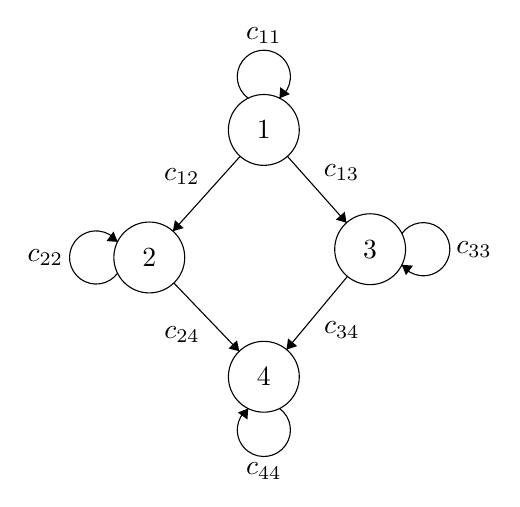
\begin{tikzpicture}[scale=0.15,
baseline={(current bounding box.center)}]
\tikzstyle{every node}+=[inner sep=0pt]
\draw [black] (36.2,-11.6) circle (3);
\draw (36.2,-11.6) node {$1$};
\draw [black] (26.5,-22.4) circle (3);
\draw (26.5,-22.4) node {$2$};
\draw [black] (45.2,-21.7) circle (3);
\draw (45.2,-21.7) node {$3$};
\draw [black] (36.2,-32.5) circle (3);
\draw (36.2,-32.5) node {$4$};
\draw [black] (34.2,-13.83) -- (28.5,-20.17);
\fill [black] (28.5,-20.17) -- (29.41,-19.91) -- (28.67,-19.24);
\draw (30.81,-15.54) node [left] {$c_{12}$};
\draw [black] (34.877,-8.92) arc (234:-54:2.25);
\draw (36.2,-4.35) node [above] {$c_{11}$};
\fill [black] (37.52,-8.92) -- (38.4,-8.57) -- (37.59,-7.98);
\draw [black] (38.2,-13.84) -- (43.2,-19.46);
\fill [black] (43.2,-19.46) -- (43.05,-18.53) -- (42.3,-19.2);
\draw (41.24,-15.19) node [right] {$c_{13}$};
\draw [black] (23.82,-23.723) arc (324:36:2.25);
\draw (19.25,-22.4) node [left] {$c_{22}$};
\fill [black] (23.82,-21.08) -- (23.47,-20.2) -- (22.88,-21.01);
\draw [black] (28.58,-24.56) -- (34.12,-30.34);
\fill [black] (34.12,-30.34) -- (33.93,-29.41) -- (33.21,-30.11);
\draw (30.82,-28.92) node [left] {$c_{24}$};
\draw [black] (43.28,-24) -- (38.12,-30.2);
\fill [black] (38.12,-30.2) -- (39.02,-29.9) -- (38.25,-29.26);
\draw (41.25,-28.54) node [right] {$c_{34}$};
\draw [black] (47.88,-20.377) arc (144:-144:2.25);
\draw (52.45,-21.7) node [right] {$c_{33}$};
\fill [black] (47.88,-23.02) -- (48.23,-23.9) -- (48.82,-23.09);
\draw [black] (37.523,-35.18) arc (54:-234:2.25);
\draw (36.2,-39.75) node [below] {$c_{44}$};
\fill [black] (34.88,-35.18) -- (34,-35.53) -- (34.81,-36.12);
\end{tikzpicture}
\end{minipage}
\break
\noindent 
Our vector $\x$ is a ML model with ML coefficient matrix 
\[ B=\begin{bmatrix}
&c_{11} &c_{12}c_{11} & c_{13}c_{11}& c_{24}c_{12}c_{11}\vee c_{34}c_{13}c_{11}\\
&0 & c_{22} & 0& c_{22}c_{24}\\
&0&0 &c_{33} & c_{33}c_{34} \\
&0& 0 & 0 & c_{44}\\
\end{bmatrix}
\]
To visualize the generation of this matrix given a graph $\d$ and weights $C$, please consult r code.


\end{document}
